%--------------------------------------
% Create title frame
\titleframe

%--------------------------------------
% Table of contents
\begin{frame}{Overview}
  \setbeamertemplate{section in toc}[sections numbered]
  \tableofcontents[hideallsubsections]
\end{frame}



%--------------------------------------

%\begin{frame}
%\frametitle{What will we learn today?}
%\begin{itemize}
%    \item Why HVDC systems are used and how they are implemented (focus on LCC)
%    \item What are LCCs
%    \item What are thyristors
%    \item Basic control principles of LCC HVDC
%    \item How to insert a point-to-point HVDC line in a power flow analysis
%\end{itemize}
%\vfill
%\note{Note that I have mainly taken material from former course "ELEC0445 - HVDC grids", but it follows the logic of Chapter 7 of Ned Mohan's book.}
%\end{frame}



\section{Overview of HVDC applications}

\begin{frame}[fragile]
\frametitle{Overview of HVDC applications}
\begin{center}
\textbf{Introduction of former course "ELEC0445 - HVDC grids".}
\end{center}
\end{frame}

\begin{frame}
\frametitle{Principle of HVDC links}
\begin{itemize}
    \item HVDC links embedded in AC systems
    \item Rely on converters:
    \begin{itemize}
        \item rectifier: from AC to DC
        \item inverter: from DC to AC
    \end{itemize}
\end{itemize}
\begin{center}
    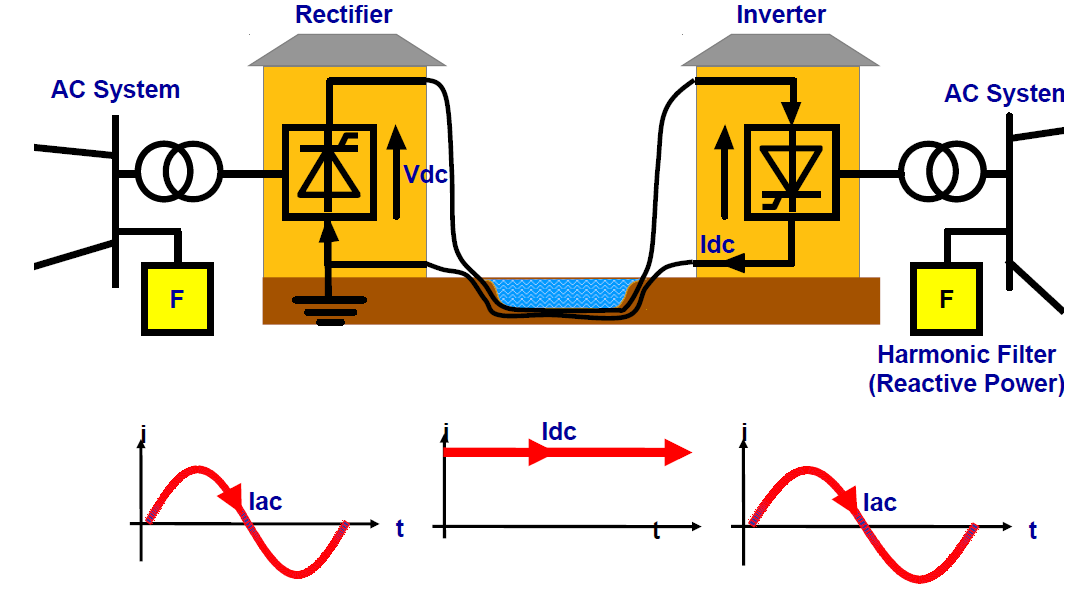
\includegraphics[width=0.5\linewidth]{images/principlesHVDC.png}
\end{center}
\end{frame}

\subsection{Historical perspective}

\begin{frame}[allowframebreaks]{Historical perspective}
\begin{itemize}
    \item At the beginning (end of 19th century): two struggling parties
    \begin{itemize}
        \item first generators producing Direct Current (DC) - Gramme, Edison
        \item first generators producing Alternating Current (AC) - Ferranti, Tesla
    \end{itemize}
    \item Have a look at the video ``War of the currents'' at \href{https://www.youtube.com/watch?v=dIfIRj0Crc8}{YouTube}.
    \item The AC system won:
    \begin{itemize}
        \item possibility to increase and lower the voltage thanks to the transformer $\Rightarrow$ transmission of higher powers possible
        \item creation of a rotating field easy with three-phase AC windings
        \item Difficulty to raise the DC voltage $\Rightarrow$ impossibility to transmit large powers with DC
        \item limitation of the power of early converters: a few kW only
        \item difficulty of interrupting a DC current.
    \end{itemize}
    \item Revival of DC technology in the ‘50s
\end{itemize}


\begin{itemize}
    \item Advances in power electronics: converters can carry larger currents through higher voltages $\Rightarrow$ higher power ratings $\Rightarrow$ transmission applications possible
    \item \textbf{1882}: Marcel Deprez (France) and Oskar Von Miller (Germany, AEG) design the first transmission link between a DC source and a DC load: \SI{15}{kW} -- \SI{2}{kV} -- \SI{56.3}{km}.
    \item See also René Thury's work
    \item \textbf{mid ‘30s}: mercury-arc valve rectifiers made available. They open the way to HVDC transmission link projects
    \item \textbf{1945}: first commercial project of HVDC transmission in Germany. Not commissioned and moved to USSR (Moscow-Kashira) in 1950: \SI{60}{MW} -- \SI{200}{kV} -- \SI{115}{km}, with buried cables.
    \item \textbf{1954}: first commercial HVDC submarine installation: from Gotland island to Sweden: \SI{20}{MW} -- \SI{100}{kV} -- \SI{98}{km}.
    \item Up to the mid ‘60s, due to its higher cost, HVDC was favoured only where AC met operational difficulties, e.g. sea crossing.
\end{itemize}


\begin{itemize}
    \item \textbf{late ‘60s}: advent of high power \textbf{thyristor}-based valve converters
    \item \textbf{1975}: 1st long-distance HVDC transmission using thyristor valve converters: Cahora Bassa in Mozambique: \SI{1920}{MW} -- \SI{533}{kV} -- \SI{1420}{km}, with overhead line
\end{itemize}
\begin{center}
    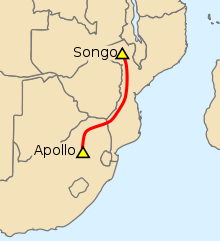
\includegraphics[width=0.2\linewidth]{images/Cahora_Bassa.png}
\end{center}
\begin{itemize}
    \item thyristor ratings have grown up to $V=\SI{9}{kV}$ and $I=\SI{4}{kA}$ (per thyristor)
    \item \textbf{late ‘90s}: high power \textbf{transistor}-based components become available: IGBT, MOSFET
    \item development of \textbf{Voltage Source Converters}. Among other advantages, they allow controlling both the active and the reactive powers at the AC terminals of an HVDC link.
\end{itemize}
\end{frame}


\subsection{Applications}

\begin{frame}
\frametitle{First application: Power transmission over long distances}
Long AC lines require reactive power compensation / voltage support and for distances larger than \SI{600}{km}-\SI{800}{km}, HVDC is more economical

Examples:
\begin{columns}
\begin{column}{0.5\linewidth}
\begin{itemize}
    \item Pacific DC inter-tie along West coast of USA: \SI{1360}{km} -- \SI{3100}{MW} -- $\pm \SI{500}{kV}$
    \item Cahora-Bassa line in Mozambique: \SI{1420}{km} -- \SI{1920}{MW} -- $\pm \SI{533}{kV}$
    \item Hydro-Québec DC line: \SI{1018}{km} -- \SI{2000}{MW} -- $\pm \SI{450}{kV}$
\end{itemize}
\end{column}
\begin{column}{0.5\linewidth}
\begin{center}
    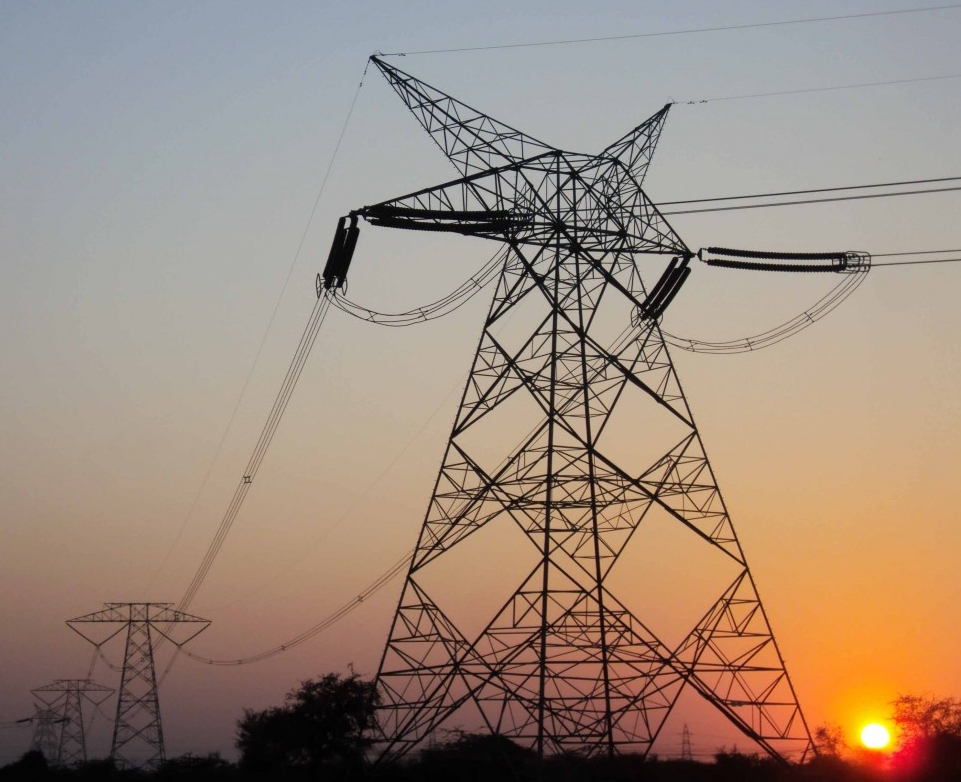
\includegraphics[width=0.7\linewidth]{images/overhead_line.jpg}
\end{center}
\end{column}
\end{columns}
\end{frame}

\begin{frame}
\frametitle{Smaller investment costs}
\begin{columns}
\begin{column}{0.5\linewidth}
\begin{center}
    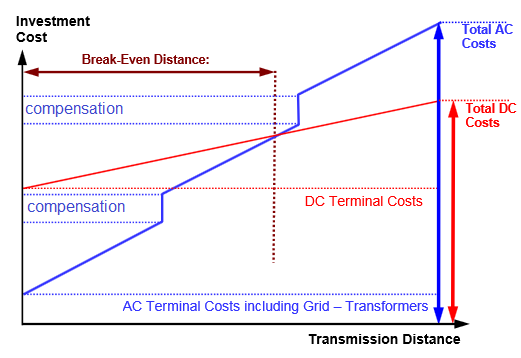
\includegraphics[width=0.7\linewidth]{images/cost.png}
\end{center}
\end{column}
\begin{column}{0.5\linewidth}
\begin{center}
    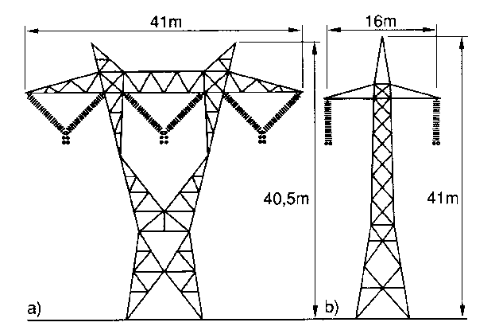
\includegraphics[width=0.7\linewidth]{images/row.png}
\end{center}
\end{column}
\end{columns}
\begin{columns}
\begin{column}{0.5\linewidth}
\begin{itemize}
    \item initial investment is higher for DC (due to converters) but
    \item with increasing distance, reactive power compensation is required for an AC line
    \item break-even distance \SI{600}{km}-\SI{800}{km}
\end{itemize}
\end{column}
\begin{column}{0.5\linewidth}
\begin{itemize}
    \item comparison of towers: same transmission capacity of \SI{3}{GW}, a) \SI{735}{kV} AC b) $\pm \SI{500}{kV}$ DC
    \item smaller Right-of-Way for DC corridor
    \item reduced footprint
\end{itemize}
\end{column}
\end{columns}
\end{frame}

\begin{frame}
\frametitle{Lower losses, higher thermal capacity}
\begin{center}
    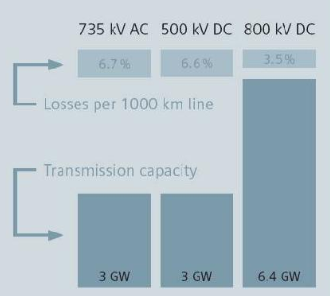
\includegraphics[width=0.3\linewidth]{images/losses.png}
\end{center}
At a similar voltage level (RMS phase-to-phase vs. DC pole-to-ground):
\begin{itemize}
    \item a DC line can transmit more than twice the power of an AC line
    \item with about half the losses of an AC line.
\end{itemize}
\end{frame}



\begin{frame}
\frametitle{Second application: submarine power transmission}
\begin{columns}
\begin{column}{0.6\linewidth}
\begin{itemize}
    \item AC cables have large capacitance. Maximal acceptable length: \SI{50}{km}-\SI{70}{km}.
    \begin{itemize}
        \item For larger distances, HVDC is the only (reasonable) solution
    \end{itemize}
    \item Examples from Europe:
    \begin{itemize}
        \item NorNed link between Norway and The Netherlands (2008): \SI{580}{km} -- \SI{700}{MW} -- $\pm \SI{450}{kV}$ (LCC type)
        \item Nemo link between Belgium and UK (2019): \SI{140}{km} -- \SI{1000}{MW} -- $\pm \SI{400}{kV}$ (VSC type)
        \item Connections of off-shore wind parks in North Sea to the continental European grid
    \end{itemize}
\end{itemize}
\end{column}
\begin{column}{0.4\linewidth}
\begin{center}
    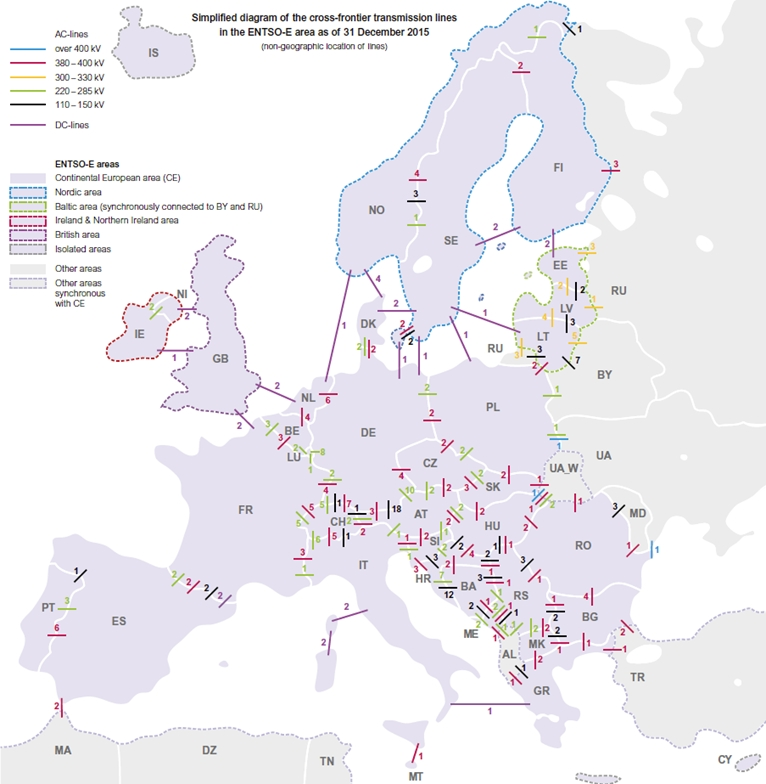
\includegraphics[width=0.8\linewidth]{images/entsoe.jpg}
\end{center}
\begin{center}
    \textit{Source ENTSOe (www.entsoe.eu)}
\end{center}
\end{column}
\end{columns}
\end{frame}



\begin{frame}
\frametitle{Third application: DC link in AC grid, for power flow control}
\begin{itemize}
    \item power flows in AC lines cannot be controlled directly
    \begin{itemize}
        \item determined by line impedances, obeying Ohm and Kirchhoff laws
        \item partially controllable by phase shifting transformers
    \end{itemize}
    \item power flows in HVDC links can be controlled directly (through the controllers of converters). This can be used:
    \begin{itemize}
        \item to limit \emph{loop flows} and overloading of AC lines
        \item to make the link participate in energy tradings.
    \end{itemize}
    \item Examples:
    \begin{itemize}
        \item ALEGrO (Aachen Liège Electric Grid Overlay) project of HVDC link between Belgium and Germany (2020): \SI{100}{km} (\SI{49}{km} in Belgium) -- \SI{1000}{MW} -- buried cable
        \item France - Spain DC interconnection: \SI{65}{km} -- buried XLPE cable -- $\pm$ \SI{320}{kV} DC -- \SI{2000}{MW}.
    \end{itemize}
\end{itemize}
\end{frame}


\begin{frame}
\frametitle{France - Spain DC interconnection}
\begin{columns}
\begin{column}{0.5\linewidth}
\begin{itemize}
    \item Can reverse power flow in 150 milliseconds (!)
    \item Investment cost: \SI{700}{M\text{\texteuro}}
\end{itemize}
\end{column}
\begin{column}{0.5\linewidth}
\begin{center}
    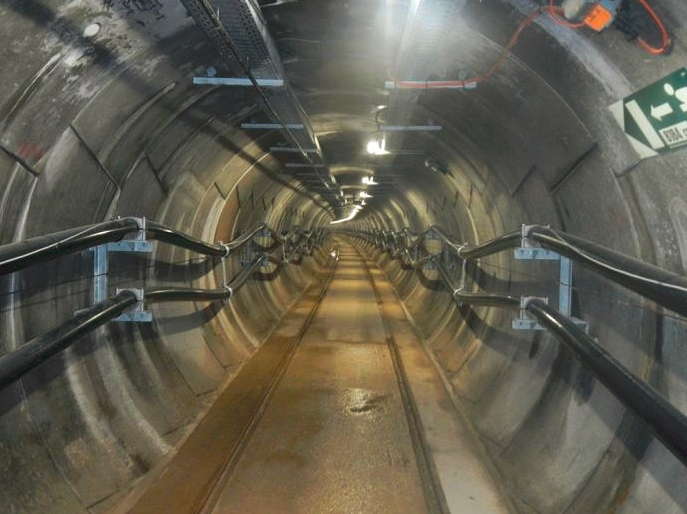
\includegraphics[width=0.4\linewidth]{images/tunnel_pyrenees.jpg}
\end{center}
\end{column}
\end{columns}
\begin{columns}
\begin{column}{0.5\linewidth}
\begin{center}
    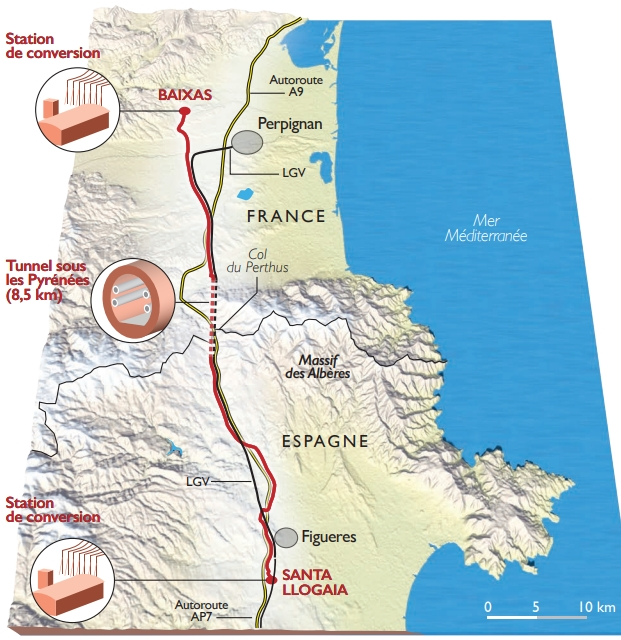
\includegraphics[width=0.5\linewidth]{images/int_France_Espagne.jpg}
\end{center}
\end{column}
\begin{column}{0.5\linewidth}
\begin{center}
    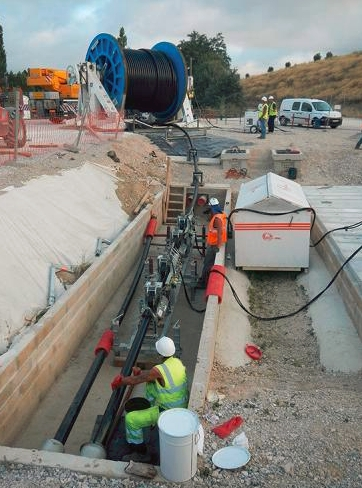
\includegraphics[width=0.4\linewidth]{images/cable_pyrenees.jpg}
\end{center}
\end{column}
\end{columns}
\end{frame}



\begin{frame}
\frametitle{Fourth application: interconnection of asynchronous AC systems}
\textit{Two AC networks with different nominal frequencies.}
Back-to-back connection (rectifier and inverter in same substation)
\begin{columns}
\begin{column}{0.5\linewidth}
\begin{itemize}
    \item Melo HVDC link between Uruguay (\SI{50}{Hz}) and Brazil (\SI{60}{Hz}): \SI{500}{MW} -- $\pm \SI{79}{kV}$
    \item Shin Shinano HVDC link between Western (\SI{60}{Hz}) and Eastern (\SI{50}{Hz}) power grids of Japan: \SI{600}{MW} -- $\pm \SI{125}{kV}$
\end{itemize}
\end{column}
\begin{column}{0.5\linewidth}
\begin{center}
    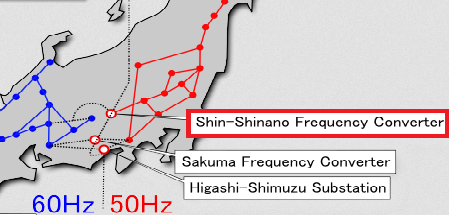
\includegraphics[width=0.8\linewidth]{images/japan.png}
\end{center}
\end{column}
\end{columns}
\end{frame}

\begin{frame}
\textit{Two AC networks with identical nominal frequency but different frequencies (not interconnected for size reasons)}
\begin{columns}
\begin{column}{0.5\linewidth}
\begin{itemize}
    \item Highgate back-to-back HVDC link between Québec and Vermont: \SI{200}{MW} -- $\pm \SI{57}{kV}$
\end{itemize}
\begin{center}
    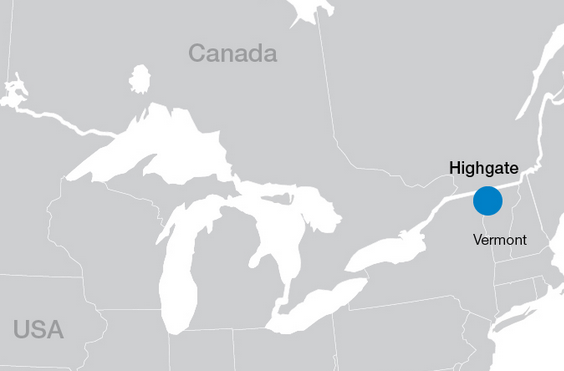
\includegraphics[width=0.5\linewidth]{images/highgate.png}
\end{center}
\begin{center}
    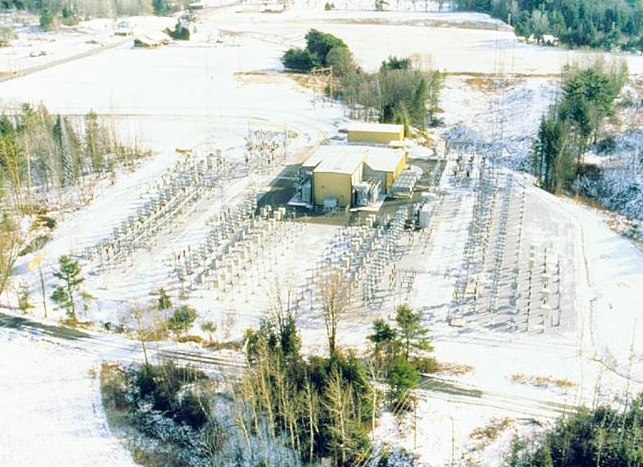
\includegraphics[width=0.5\linewidth]{images/highgate2.png}
\end{center}
\end{column}
\begin{column}{0.5\linewidth}
\begin{itemize}
    \item McNeil HVDC link between Alberta and Saskatchewan: \SI{150}{MW} -- $\pm \SI{42}{kV}$
\end{itemize}
\begin{center}
    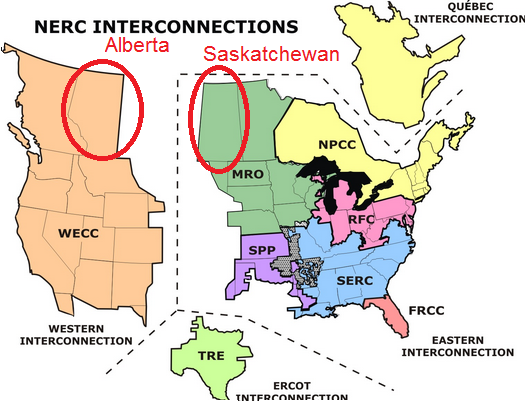
\includegraphics[width=0.7\linewidth]{images/usa.png}
\end{center}
\end{column}
\end{columns}
\end{frame}


\begin{frame}[allowframebreaks]{Fifth application: Multiterminal DC grids}
\textit{Radial} DC link with AC/DC converter(s) connected at intermediate points.
\begin{columns}
\begin{column}{0.5\linewidth}
\begin{center}
    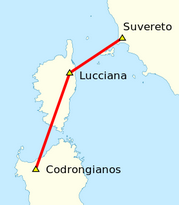
\includegraphics[width=0.6\linewidth]{images/mtdc2.png}
\end{center}
\end{column}
\begin{column}{0.5\linewidth}
\begin{itemize}
    \item A few systems are in operation today with proven technology.
    \begin{itemize}
        \item example: the Sardinia-Corsica-Italy link (SACOI)
3 terminals. The 2-terminal Italy-Sardinia link was initially built, and the Corsica terminal installed at a later stage
    \end{itemize}
    \item more elaborate control scheme than for a two-terminal link.
\end{itemize}
\end{column}
\end{columns}
\begin{columns}
\begin{column}{0.5\linewidth}
\begin{itemize}
    \item Another application: collect power from off-shore wind parks located along a DC link between two on-shore terminals.
\end{itemize}
\end{column}
\begin{column}{0.5\linewidth}
\begin{center}
    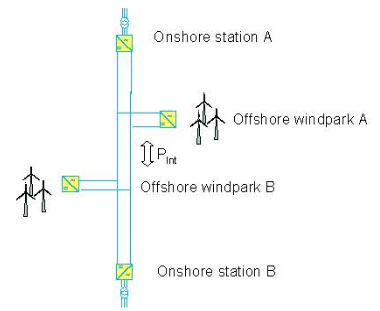
\includegraphics[width=0.8\linewidth]{images/mtdc1.png}
\end{center}
\end{column}
\end{columns}
\end{frame}


\begin{frame}
\frametitle{Meshed DC grids}
\begin{columns}
\begin{column}{0.5\linewidth}
\begin{itemize}
    \item Still at research level
    \item Typical targeted application: (i) collect power from off-shore wind parks, and (ii) allow power exchanges between on-shore grids.
\end{itemize}
Main technological challenges:
\begin{itemize}
    \item identification of faults in DC grid (to isolate only the faulted branch)
    \item DC circuit breaker to interrupt the DC fault current.
\end{itemize}
\end{column}
\begin{column}{0.5\linewidth}
\begin{center}
    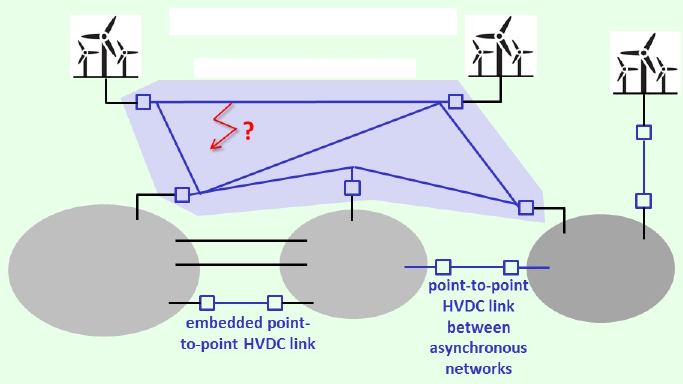
\includegraphics[width=0.8\linewidth]{images/supergrid.png}
\end{center}
\end{column}
\end{columns}
\end{frame}



\begin{frame}
\frametitle{Two technologies}
\begin{columns}
\begin{column}{0.6\linewidth}
\textbf{Line Commuted Converters (LCC)}
\begin{itemize}
    \item large power ratings
    \item large harmonics filters
    \item requires a strong enough AC grid
    \item active power is controlled
    \item always consumes reactive power
    \item cannot be used as off-shore terminal to collect wind power
    \item cheaper (but VSC is a fast evolving technology)
    \item less commutation losses than VSC
    \item but possible commutation failure
\end{itemize}
\end{column}
\begin{column}{0.4\linewidth}
\textbf{Voltage Source Converters (VSC)}
\begin{itemize}
    \item lower power ratings (but fast growing technology)
    \item less harmonic filters needed
    \item can operate with a weak AC grid
    \item active \textbf{and reactive} powers can be controlled
    \item can be used as off-shore terminal to collect wind power
    \item black start capability
\end{itemize}
\end{column}
\end{columns}
\end{frame}


\begin{frame}
\frametitle{LCC technology}
\begin{center}
    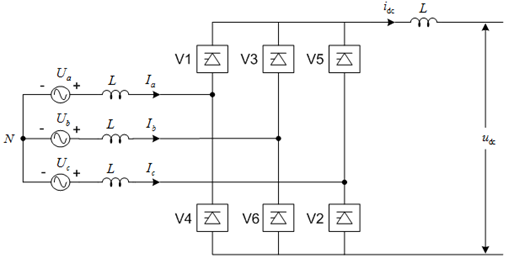
\includegraphics[width=0.4\linewidth]{images/lcc.png}
\end{center}
\begin{itemize}
    \item based on thyristors, used as switches closed with delay
    \item thyristor commutation synchronized with grid voltage (hence the term ``line commutated'')
    \item also referred to as ``Current Source Converter'' or ``classic HVDC''
    \item DC current cannot be reversed (due to thyristors). Hence, power is reversed by reversing the DC voltage polarity.
\end{itemize}
\end{frame}

\begin{frame}
\frametitle{VSC technology}
Based on Insulated Gate Bipolar Transistors (IGBT), used as interrupteurs \textit{self-commutating} switches.

Two topologies:
\begin{columns}
\begin{column}{0.6\linewidth}
\begin{center}
    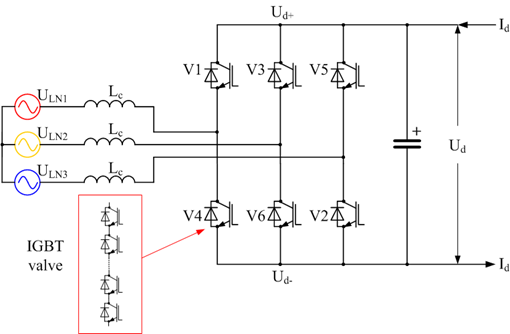
\includegraphics[width=0.5\linewidth]{images/pwm.png}\\
Pulse Width Modulation (PWM)
\end{center}
\end{column}
\begin{column}{0.4\linewidth}
\begin{center}
    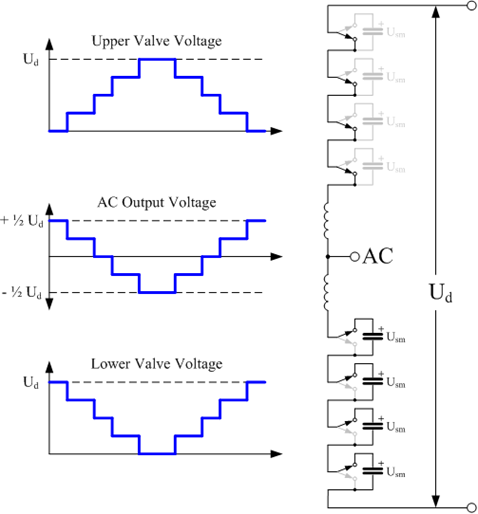
\includegraphics[width=0.5\linewidth]{images/mmc.png} \\
Modular Multilevel Converter (MMC)
\end{center}
\end{column}
\end{columns}
Power is reversed by reversing the current.
\end{frame}




\section{Components of an LCC HVDC link}

\begin{frame}[fragile]
\frametitle{Components of an LCC HVDC link}
\begin{center}
\textbf{Extract of chapter 1 of former course "ELEC0445 - HVDC grids".}
\end{center}
\end{frame}

\begin{frame}
\frametitle{A typical LCC HVDC system}
\begin{center}
    \includegraphics[width=1.0\linewidth]{images/typical-HVDC.png}
\end{center}
\end{frame}

\begin{frame}{Converters}
\begin{center}
    \includegraphics[width=0.5\linewidth]{images/typical-HVDC1.png}
\end{center}
\begin{itemize}
    \item one converter at each terminal: the sending power end acts as a rectifier, the receiving power end as an inverter
    \begin{itemize}
        \item each converter includes one or several thyristor \textbf{bridges}
        \item each bridge is made up of \textbf{6} thyristor {valves}
        \item each thyristor valve contains \textbf{hundreds of individual thyristors}
    \end{itemize}
\end{itemize}
\end{frame}



\begin{frame}{Converter transformers}
\begin{center}
    \includegraphics[width=0.5\linewidth]{images/typical-HVDC2.png}
\end{center}
\begin{itemize}
    \item most generally equipped with load tap changers. The transformer ratios are adjusted to optimize the HVDC link operation
    \item designed to operate with high harmonic currents
    \begin{itemize}
        \item generally more expensive than typical transmission transformers of the same rating
    \end{itemize}
\end{itemize}
\end{frame}

\begin{frame}{Smoothing reactors on the DC side}
\begin{center}
    \includegraphics[width=0.5\linewidth]{images/typical-HVDC3.png}
\end{center}
\begin{itemize}
    \item aimed at limiting the DC current variations
    \begin{itemize}
        \item designed considering response to DC faults and commutation failures
        \item typical values of inductance: \SI{0.1}{H} to \SI{0.5}{H}
        \item air-core, natural air cooling type
    \end{itemize}
\end{itemize}
\end{frame}


\begin{frame}{Harmonic filters}
\begin{center}
    \includegraphics[width=0.5\linewidth]{images/typical-HVDC4.png}
\end{center}
\begin{itemize}
    \item aimed at filtering the harmonics generated by the AC/DC conversion
    \begin{itemize}
        \item most important harmonics to eliminate: 11th, 13th, 23rd and 25th (for converters with two bridges)
        \item some HVDC systems are also equipped with filters on the DC side
    \end{itemize}
\end{itemize}
\end{frame}

\begin{frame}{Reactive power compensation}
\begin{center}
    \includegraphics[width=0.5\linewidth]{images/typical-HVDC5.png}
\end{center}
\begin{itemize}
    \item the converters consume reactive power (around 60\% of power rating)
    \item that reactive power varies with the active power level
    \item a large part of the reactive compensation comes from the filter banks
    \item the remaining part is supplied by switchable capacitor banks
\end{itemize}
\end{frame}

\begin{frame}{Control and communication systems}
\begin{center}
    \includegraphics[width=0.5\linewidth]{images/typical-HVDC6.png}
\end{center}
\begin{itemize}
    \item each terminal has a control system with multiple hierarchical layers: control of resp. the DC current, the DC voltage, the thyristors, etc.
    \item a dedicated communication link is needed between both terminals to optimize system operation
\end{itemize}
\end{frame}



\section{Thyristor valves}

\begin{frame}[fragile]
\frametitle{Thyristor valves}
\begin{center}
\textbf{A summary of chapter 2 of former course "ELEC0445 - HVDC grids".}
\end{center}
\end{frame}

\begin{frame}[allowframebreaks]{The thyristor}
\begin{itemize}
    \item Essential component of HVDC valves in the LCC technology
    \item operates as a controllable diode
    \item can have high power ratings: up to \SI{8.5}{kV}, \SI{4500}{A} capability
    \item is robust and efficient.
\end{itemize}
Four-layer, three-terminal device.
\begin{columns}
\begin{column}{0.5\linewidth}
Three $pn$ junctions $J_1$, $ J_2$, $J_3$
\begin{center}
    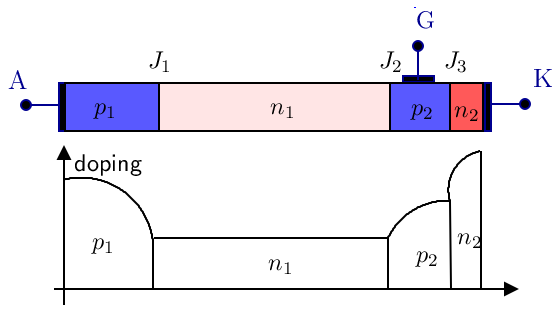
\includegraphics[width=1.0\linewidth]{images/thyristor1.png}
\end{center}
\end{column}
\begin{column}{0.5\linewidth}
\begin{itemize}
    \item equivalent to two bipolar transistors
    \item assume $V_{AK}>0$ and inject $I_G$
    \item both transistors remain in saturation even if $I_G$ is suppressed
\end{itemize}
\begin{center}
    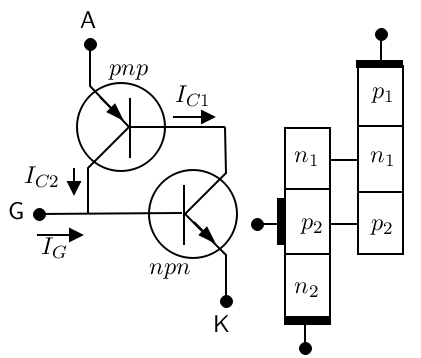
\includegraphics[width=0.5\linewidth]{images/thyristor2.png}
\end{center}
\end{column}
\end{columns}
\end{frame}

\begin{frame}[allowframebreaks]{Usage of a thyristor}
A thyristor can be used as a controllable bistable switch
\begin{itemize}
    \item the control is performed by injecting a current at the gate input
    \item the thyristor is \textit{ON} and conducts when it is forward biased and the gate receives a current pulse
    \item the thyristor keeps on conducting as long as it is forward biased
    \item the thyristor is turned \textit{OFF} when the anode current falls below the holding current threshold IH or when it is reverse biased
    \item the thyristor remains in blocking mode until it is triggered by a new gate pulse current
\end{itemize}

The process of turning OFF is called commutation
\begin{itemize}
    \item when commutating, the thyristor cannot immediately withstand a forward voltage; it should remain reverse biased for a minimum time, otherwise \textit{commutation failure} can take place.
\end{itemize}
\end{frame}

\begin{frame}{Modes of operation of the thyristor}
Three modes of operation depending on:
\begin{itemize}
    \item the sign of the anode - cathode voltage $v_{AK}$
    \item whether a current $I_G$ is injected at the gate terminal
\end{itemize}
\end{frame}
\begin{frame}{1. A \textit{reverse voltage $v_{AK}<0$} is applied}
\begin{itemize}
    \item Junction $J_2$ is in \textit{forward} bias mode
    \item junctions $J_1$ and $J_3$ are in \textit{reverse} bias mode
    \item the thyristor acts as a diode in reverse bias mode; it is in \textit{off-state}
    \item breakdown occurs when $v_{AK}$ is more negative than the \textit{reverse breakdown voltage} $V_{BR}$. Most often this is associated with junction $J_1$
    \item in HVDC applications, the breakdown mode must be avoided since it can lead to material destruction.
    \item hence, thyristors with high $|V_{BR}|$ values must be used, and measures taken to limit the avalanche current.
\end{itemize}

\end{frame}
\begin{frame}{2. A \textit{forward voltage $v_{AK}>0$} is applied}
    
\begin{columns}
\begin{column}{0.45\linewidth}
\begin{itemize}
    \item Junctions $J_1$ and $J_3$ are \textit{forward} in bias mode
    \item junction $J_2$ is in \textit{reverse} bias mode
    \item the thyristor behaves as a diode in reverse bias mode; it is in \textit{off-state}
    \item breakdown occurs when $v_{AK}$ is larger than the forward breakdown voltage of junction $J_2$.
\end{itemize}
\end{column}
\begin{column}{0.55\linewidth}
\begin{center}
    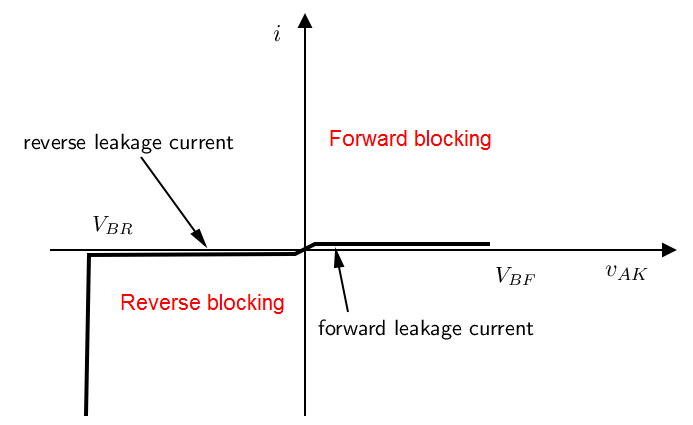
\includegraphics[width=0.99\linewidth]{images/thyristor3.png}
\end{center}
\end{column}
\end{columns}
\end{frame}

\begin{frame}{3. A \textit{forward voltage $v_{AK}>0$} is applied and \textit{a current $I_g$ is injected}}
\begin{itemize}
    \item the current injection results in an avalanche process
    \item ``as if'' layer $p_2$ would become of $n$-type. Hence, the thyristor behaves as a $pn$ diode in forward bias mode: it switches to \textit{on-state}
    \item the thyristor resistance is dramatically reduced (from \SI{1}{\mega\ohm} to \SI{0.1}{\ohm})
    \item the larger $I_G$, the smaller the value of $v_{AK}$ needed to initiate the avalanche.
\end{itemize}
\end{frame}

\begin{frame}
\frametitle{Operation of the thyristor in on-state}

\begin{columns}
\begin{column}{0.4\linewidth}
\begin{center}
    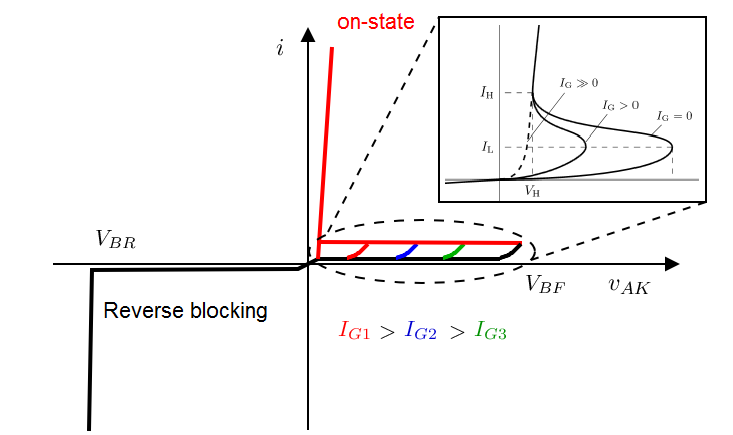
\includegraphics[width=\linewidth]{images/thyristor4.png}
\end{center}
\end{column}
\begin{column}{0.6\linewidth}
\begin{itemize}
    \item Once the anode current $i$ reaches $I_L$, the \textit{latching curent}, the thyristor switches to on-state
    \item once the thyristor is in on-state, the gate current can be removed
    \item the gate current is usually a short pulse lasting \SI{10}{}-\SI{50}{\mu s}
    \item if $i$ falls below $I_H$, the \textit{holding curent}, the thyristor switches to off-state.
\end{itemize}
\end{column}
\end{columns}
\textbf{Commutation is not instantaneous} -> dynamics -> and care must be taken with applied currents and voltages -> snubber circuits
\end{frame}

\begin{frame}
\frametitle{The ideal characteristic}
\begin{columns}
\begin{column}{0.45\linewidth}
\begin{center}
    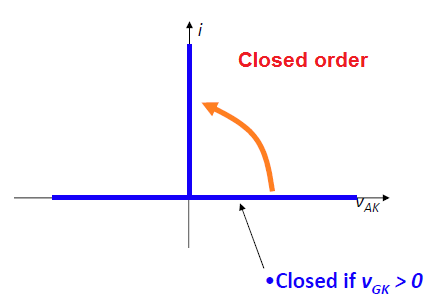
\includegraphics[width=1.0\linewidth]{images/thyr-id2.png}
\end{center}
\end{column}
\begin{column}{0.45\linewidth}
\begin{center}
    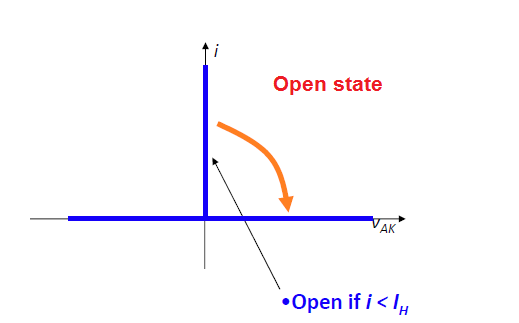
\includegraphics[width=1.0\linewidth]{images/thyr-id1.png}
\end{center}
\end{column}
\end{columns}
\begin{itemize}
    \item Closed order given by gate current
    \item in open state, $V_{BR}$ and $V_{BF}$ are assumed infinite
    \item when the thyristor conducts, a zero internal resistance is assumed
    \item when the thyristor conducts, a zero terminal voltage is assumed.
\end{itemize}
\end{frame}

\begin{frame}
\frametitle{Thyristor valves}
\begin{columns}
\begin{column}{0.5\linewidth}
Thyristor modules (i.e. thyristor + snubber circuit + voltage balancing circuits) are associated in series to form a thyristor valve.
\begin{itemize}
    \item Objective: reach the HVDC link
    \item voltage rating:
    \begin{itemize}
        \item thyristor: up to \SI{5}{kV} to \SI{9}{kV}
        \item HVDC link: \SI{500}{kV} to \SI{800}{kV}
    \end{itemize}
\end{itemize}
\vspace{2mm}
\textit{On the right: A \SI{2000}{A}, \SI{250}{kV} high voltage direct current (HVDC) thyristor valve at Manitoba Hydro's Henday converter station. Photo taken April 2001. Source: Wikipedia.}
\end{column}
\begin{column}{0.5\linewidth}
\begin{center}
    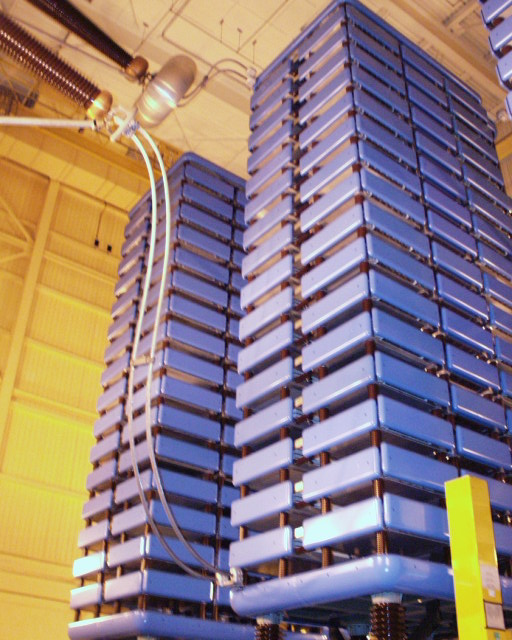
\includegraphics[width=0.7\linewidth]{images/Manitoba_Hydro-BipoleII_Valve.jpg}
\end{center}

\end{column}
\end{columns}
\end{frame}




\section{Operation of the LCC line}

\begin{frame}[fragile]
\frametitle{Operation of the LCC line}
\begin{center}
\textbf{A summary of chapter 3 of former course "ELEC0445 - High Voltage Direct Current grids".}
\end{center}
\end{frame}

\begin{frame}
\frametitle{Diode based rectifier}
\begin{columns}
\begin{column}{0.5\linewidth}
\begin{center}
    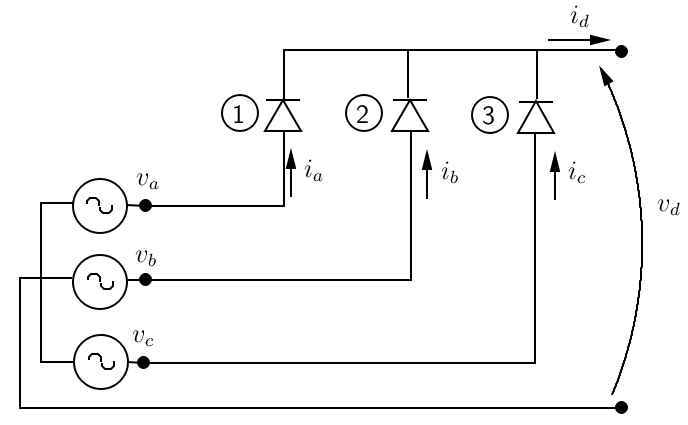
\includegraphics[width=1.0\linewidth]{images/3pulseconv.png}
\end{center}
\end{column}
\begin{column}{0.5\linewidth}
\begin{center}
    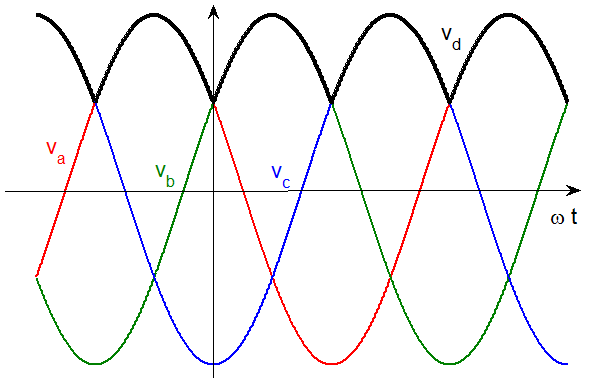
\includegraphics[width=0.7\linewidth]{images/3pulsevred.png}
\end{center}
\begin{center}
    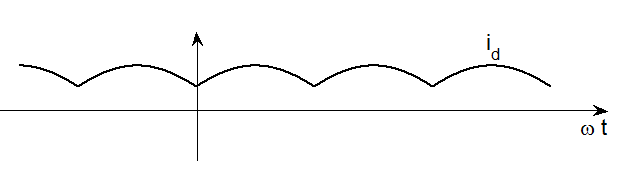
\includegraphics[width=0.7\linewidth]{images/3pulseired.png}
\end{center}
\end{column}
\end{columns}
Without filtering, we already have a relatively good rectification.
\end{frame}

\begin{frame}
To get a more constant current, we use smoothing reactors in series. The bigger $L_d$, the more constant the current.
Hence we suppose $I_d$ is constant, and the currents in the 3 phases on the AC side look like:
\begin{columns}
\begin{column}{0.5\linewidth}
\begin{center}
    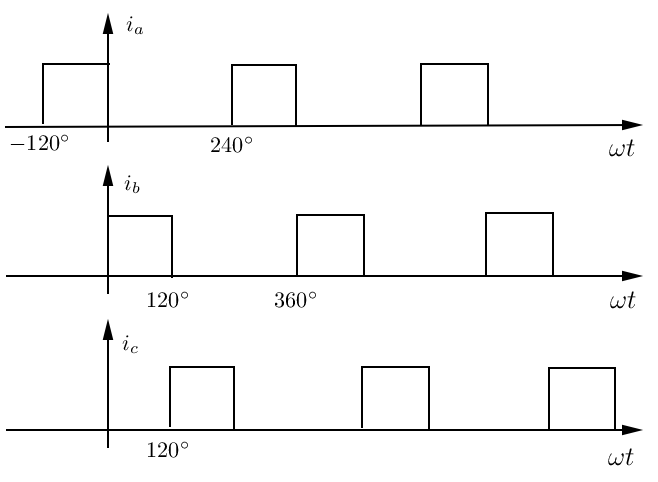
\includegraphics[width=\linewidth]{images/currents3pulse.png}
\end{center}
\end{column}
\begin{column}{0.5\linewidth}
Note that in practice, as there are inductors in the system, currents cannot vary abruptly, and there is a \textit{commutation overlap} (two of the three diodes conducting simultaneously), hence an angle $\mu$ and a voltage reduction. We'll neglect this in the sequel (to keep it simple), but this is important in practice.
\end{column}
\end{columns}
\end{frame}

\begin{frame}
\frametitle{The thyristor-based 6-pulse rectifier with \textit{no ignition delay}}
In this case Thyristor = Diode (natural conduction)
\begin{columns}
\begin{column}{0.4\linewidth}
\begin{center}
    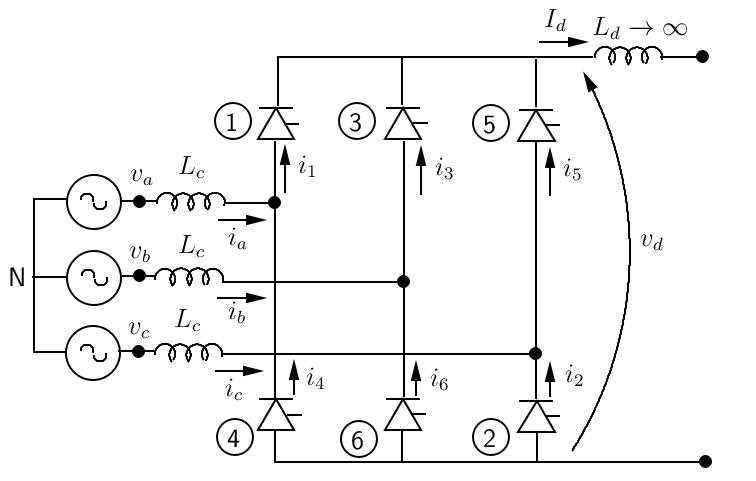
\includegraphics[width=1.0\linewidth]{images/6pulsebridge.png}
\end{center}
\end{column}
\begin{column}{0.55\linewidth}
\begin{center}
    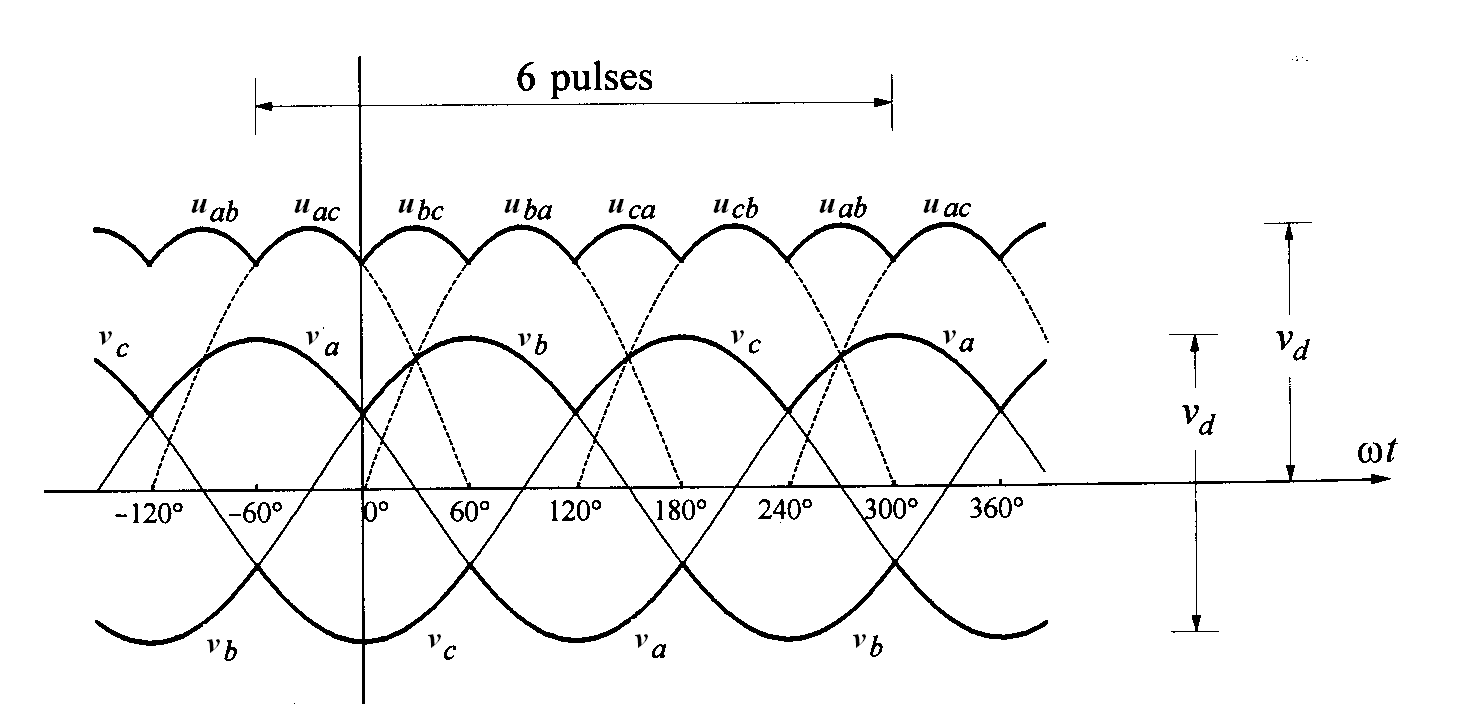
\includegraphics[width=1.0\linewidth]{images/6pulsevolt1.png}
\end{center}
\end{column}
\end{columns}

\begin{block}{Average direct voltage}
The {average direct voltage} is $V_{d0} = \frac{3\sqrt{2}}{\pi} U \approx 1.35 U$.

Exercise: verify this formula, what is exactly $U$ in this case? 
\end{block}



\end{frame}

\begin{frame}[allowframebreaks]{Solution}
    Let $x = \omega t$.

    The average direct voltage value is given by $$ V_{d0}=\frac{1}{2\pi}\int_{0}^{2\pi} v_d(x) dx$$

    Since $v_d(t)$ repeats 6 times over a period of $2 \pi$, we can equivalently write 
    $$ V_{d0}=\frac{6}{2\pi}\int_{\pi/3}^{2\pi/3} v_d(x) dx$$
    arbitrarily selecting the interval $[{\pi/3}, {2\pi/3}]$ of length $\pi/3$ where $v_d(x) = \sqrt{2} U sin(x)$

    Hence $$ V_{d0}=\frac{6}{2\pi}\int_{\pi/3}^{2\pi/3} \sqrt{2} U \sin(x) dx = -\frac{3\sqrt{2}}{\pi} U \left(cos \frac{2\pi}{3} - cos \frac{\pi}{3}\right) = \frac{3\sqrt{2}}{\pi} U$$

    $U$ is the rms line-to-line voltage.

\end{frame}


\begin{frame}
\begin{block}{Average direct voltage with an ignition delay $\alpha$}
The {average direct voltage} is $$V_{d} = V_{d0} \cos \alpha$$

Exercise: verify this formula. 
\end{block}

\begin{columns}
\begin{column}{0.5\linewidth}
    \begin{center}
    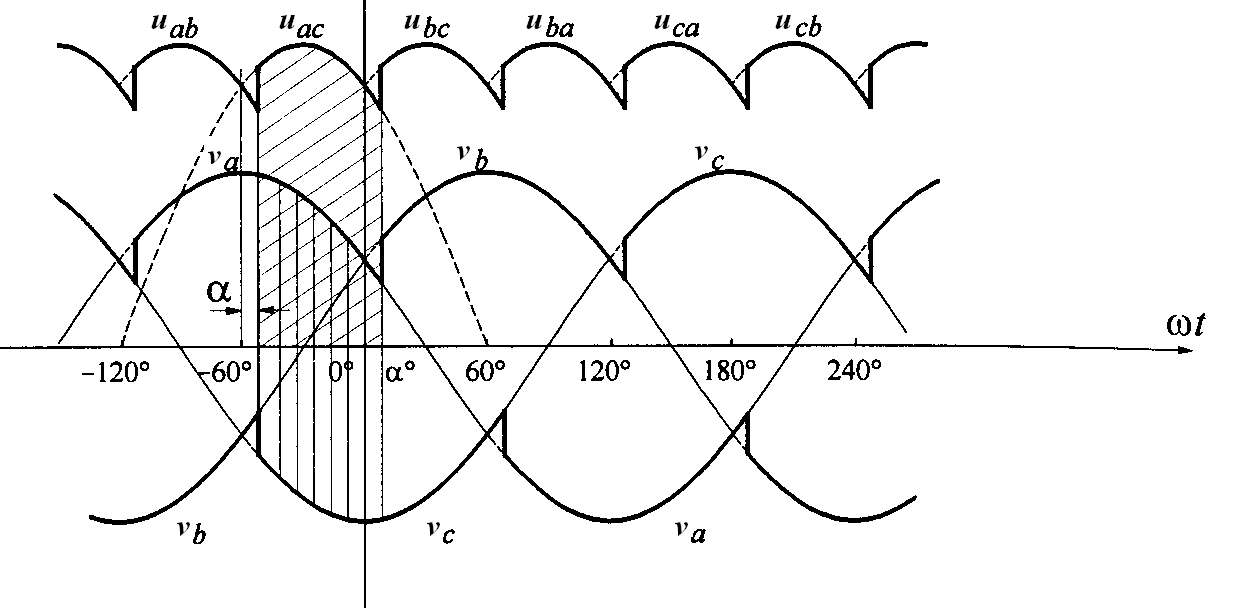
\includegraphics[width=\linewidth]{images/6pulse-alpha1.png}
\end{center}
\end{column}
\begin{column}{0.5\linewidth}
The ignition can be delayed up to $\alpha=180^\circ$
\begin{itemize}
    \item for instance: switching from valve 1 to valve 3 is possible as long as $v_a < v_b$.
    \item After that, valve 3 is in reverse blocking mode.
\end{itemize}
\end{column}
\end{columns}
%Waveforms in a rectified multiple thyristor circuit controlling an AC current. Trace red: load (output) voltage. Trace blue: trigger voltage. Source: Wikipedia (Thyristor).
\end{frame}

\begin{frame}[allowframebreaks]{Solution}
The average DC voltage is the average of the instantaneous voltage over one period. 
We integrate the instantaneous voltage over a $\frac{\pi}{3}$ interval, taking into account the firing angle $\alpha$. 
The instantaneous output voltage is a segment of the line-to-line voltage, which can be modeled as $v_{d}(\omega t) = \sqrt{2}U\sin(\omega t)$. 
The conduction interval spans from $\omega t = \frac{\pi}{3} + \alpha$ to $\omega t = \frac{2\pi}{3} + \alpha$.

The formula for the average value is:
$$ V_d = \frac{1}{\text{period}} \int_{\text{interval}} v_d(\omega t) d(\omega t) $$
Substituting the values:
$$ V_d = \frac{1}{\pi/3} \int_{\pi/3 + \alpha}^{2\pi/3 + \alpha} \sqrt{2}U \sin(\omega t) d(\omega t) $$


We solve the definite integral:
$$ V_d = \frac{3\sqrt{2}U}{\pi} \left[ -\cos(\omega t) \right]_{\pi/3 + \alpha}^{2\pi/3 + \alpha} $$
$$ V_d = -\frac{3\sqrt{2}U}{\pi} \left( \cos(2\pi/3 + \alpha) - \cos(\pi/3 + \alpha) \right) $$


Using the trigonometric identity $\cos(A+B) = \cos A \cos B - \sin A \sin B$:
$$ \cos(2\pi/3 + \alpha) = \cos\left(\frac{2\pi}{3}\right)\cos(\alpha) - \sin\left(\frac{2\pi}{3}\right)\sin(\alpha) = -\frac{1}{2}\cos(\alpha) - \frac{\sqrt{3}}{2}\sin(\alpha) $$
$$ \cos(\pi/3 + \alpha) = \cos\left(\frac{\pi}{3}\right)\cos(\alpha) - \sin\left(\frac{\pi}{3}\right)\sin(\alpha) = \frac{1}{2}\cos(\alpha) - \frac{\sqrt{3}}{2}\sin(\alpha) $$


We substitute these results back into the equation for $V_d$:
$$ V_d = -\frac{3\sqrt{2}U}{\pi} \left[ \left(-\frac{1}{2}\cos(\alpha) - \frac{\sqrt{3}}{2}\sin(\alpha)\right) - \left(\frac{1}{2}\cos(\alpha) - \frac{\sqrt{3}}{2}\sin(\alpha)\right) \right] $$
$$ V_d = -\frac{3\sqrt{2}U}{\pi} \left[ -\frac{1}{2}\cos(\alpha) - \frac{\sqrt{3}}{2}\sin(\alpha) - \frac{1}{2}\cos(\alpha) + \frac{\sqrt{3}}{2}\sin(\alpha) \right] $$
$$ V_d = -\frac{3\sqrt{2}U}{\pi} \left[ -\cos(\alpha) \right] $$

This gives us the final formula for the average output voltage:
$$ V_d = \frac{3\sqrt{2}U}{\pi} \cos(\alpha) $$
\end{frame}

\begin{frame}
\frametitle{Average direct voltage and power factor}
Since $V_{d} = V_{d0} \cos \alpha$, $V_d$ may take values from $V_{d0}$ down to $-V_{d0}$
\begin{itemize}
    \item positive values of $V_d$ ($0 < \alpha < 90^{\circ}$):
    \begin{itemize}
        \item \textbf{Rectifier operation}. Power flows from AC to DC since $V_d I_d > 0$.
    \end{itemize}
    \item negative values of $V_d$ ($90 < \alpha < 180^{\circ}$):
    \begin{itemize}
        \item \textbf{Inverter operation}. Power flows from DC to AC since $V_d I_d < 0$.
    \end{itemize}
    
\end{itemize}
\begin{block}{Power factor}
Without accounting for commutation delays, it can be shown that
$$\cos \phi = \cos \alpha$$    (See \cite{padiyar1990hvdc}, page 49, conservesion of power, AC to DC.)
\end{block}
\end{frame}



\section{Control}


\begin{frame}
    \frametitle{Introduction}

    \begin{itemize}
        \item HVDC links allow rapid control of transmitted power by playing on the firing angles.
        \item The control system is very complex, with many layers.  
        \item We cover here the very basic principles.
        \item See Chapter 4 in \cite{padiyar1990hvdc}.
    \end{itemize}
\end{frame}

\begin{frame}[allowframebreaks]{The HVDC link, its equivalent circuit and its voltage profile}


\begin{columns}
\begin{column}{0.6\linewidth}
\begin{center}
    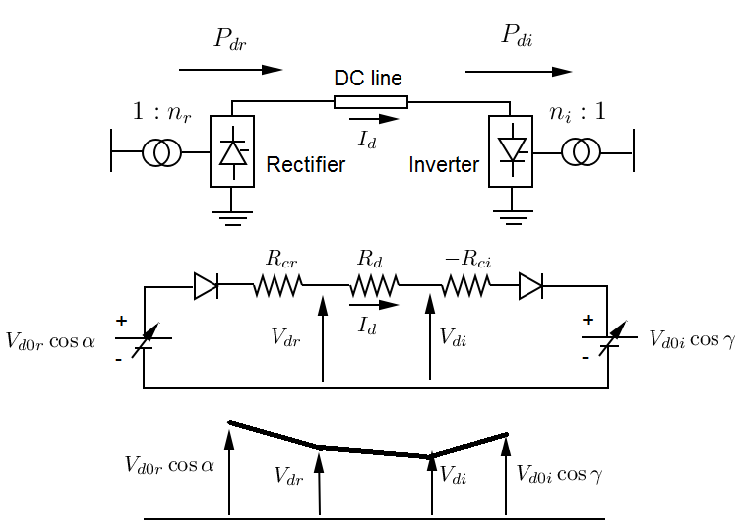
\includegraphics[width=\linewidth]{images/HVDC-equiv.png}
\end{center}
\end{column}
\begin{column}{0.4\linewidth}
Thus,
$$I_d=\frac{V_{d0r}\cos \alpha - V_{d0i} \cos \gamma}{R_{cr} + R_d - R_{ci}}$$
and
$$P_{dr} = V_{dr}I_d,$$ $$P_{di} = V_{di}I_d = P_{dr} - R_d I_d^2$$
\end{column}
\end{columns}

Since $R_{cr} + R_d - R_{ci}$ is typically small, sudden voltage variations can lead to large current variation if firing angles are kept constant.
Hence it is important to regulate DC voltages close to their nominal value: 
\begin{itemize}
    \item high enough to minimize the losses
    \item small enough to avoid damages (thyristors)
\end{itemize}
\end{frame}

\begin{frame}
\frametitle{Available controls}
\begin{columns}
\begin{column}{0.5\linewidth}
We thus have
$$ V_{dr} = V_{d0r} \cos \alpha - R_{cr} I_d $$
$$ V_{di} = V_{d0i} \cos \gamma - R_{ci} I_d $$
$$ V_{dr} = V_{di} + R_d I_d $$
and as established previously
$$V_{d0r} = \frac{3 \sqrt{2}}{\pi} n_r U_r $$
$$V_{d0i} = \frac{3 \sqrt{2}}{\pi} n_i U_i$$
\end{column}
\begin{column}{0.5\linewidth}
Available controls are used in complementary manner:
\begin{itemize}
    \item (fast) the internal DC voltage $V_{d0r}\cos \alpha$ (resp. $V_{d0i}\cos \gamma$) by adjusting the ignition angle $\alpha$
     (resp. the extinction angle $\gamma$).
    \item (slow) the AC voltages of the converters through the transformer ratios $n_r$ and $n_i$.
\end{itemize}
\end{column}
\end{columns}
\end{frame}

\begin{frame}
\frametitle{Remarks}
Attention must be paid to:
\begin{itemize}
    \item avoiding too low a current $I_d$ (unstable commutation)
    \item avoiding too high a current $I_d$ (overload of valves)
    \item having a stable HVDC link operation in spite of variations of AC voltages.
\end{itemize}
The power $P_{dr}$ (or $P_{di}$) can be controlled instead of the current $I_d$.
\end{frame}

\begin{frame}
\frametitle{Control principle}
Overall principle:
\begin{itemize}
    \item the regulations of resp. $V_d$ and $I_d$ are performed by the terminals separately
    \item this does not require fast exchange of information between both terminals
    \begin{itemize}
        \item only when the respective roles of the rectifier and the inverter change
    \end{itemize}
    \item Under normal operation:
    \begin{itemize}
        \item the rectifier maintains a Constant Current (CC) $I_d$ mode (increase power transfer by decreasing $\alpha$, which imporves the power factor, and minimizes reactive power consumption)
        \item the inverter maintains Constant Extinction Angle (CEA) $\gamma$ mode, above the minumum value required to avoid commutation failure, for economical reasons.
    \end{itemize}
\end{itemize}
\end{frame}

\begin{frame}
\frametitle{Ideal steady-state $V-I$ characteristics:}
\begin{columns}
\begin{column}{0.45\linewidth}
\begin{center}
    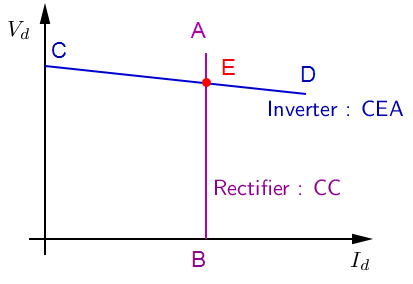
\includegraphics[width=\linewidth]{images/control1.png}
\end{center}
\end{column}
\begin{column}{0.55\linewidth}
\begin{itemize}
    \item Rectifier characteristic: $I_d = $ constant
    \item Inverter characteristic: from previous equations
    $$V_{dr}=V_{d0i}\cos \gamma +(R_d -R_{ci})I_d$$
    generally, $R_{ci}$ is slightly larger than $R_d$ and the characteristic has a small negative slope
    \item Operating state: point \textbf{E} at the intersection of the two characteristics
\end{itemize}
\end{column}
\end{columns}
\end{frame}

\begin{frame}{Exercise}
    Consider a HVDC link of  \SI{1000}{MW}, $\pm$ \SI{450}{kV}, with  $R_{cr} = \frac{3}{8} \Omega$, $R_{ci} = \frac{3}{8} \Omega$, $R_{d} = \frac{1}{4} \Omega$.
    Neglect the transformers (assume $n=1$ at the rectifier and inverter sides).
    \begin{itemize}
        \item What is the maximal value $I_d^{\max}$ of $I_d$?
        \item If $I_d = 0.5 I_d^{\max}$, what are possible values of $\alpha$ and $\gamma$?
        \item What is the voltage drop along the DC section?  
    \end{itemize}

\end{frame}

\section{HVDC in the power flow analysis}

\begin{frame}[allowframebreaks]{A simple implementation for point to point HVDC}

\begin{columns}
\begin{column}{0.5\linewidth}
From \href{https://pandapower.readthedocs.io/en/latest/elements/dcline.html}{PandaPower \cite{thurner2018pandapower} documentation}, 
a DC line
\begin{center}
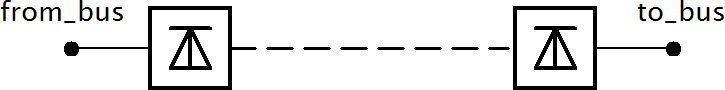
\includegraphics[width=1.0\linewidth]{images/dcline1.png}
\end{center}
is modelled as two generators in the loadflow:
\end{column}
\begin{column}{0.5\linewidth}
\begin{center}
    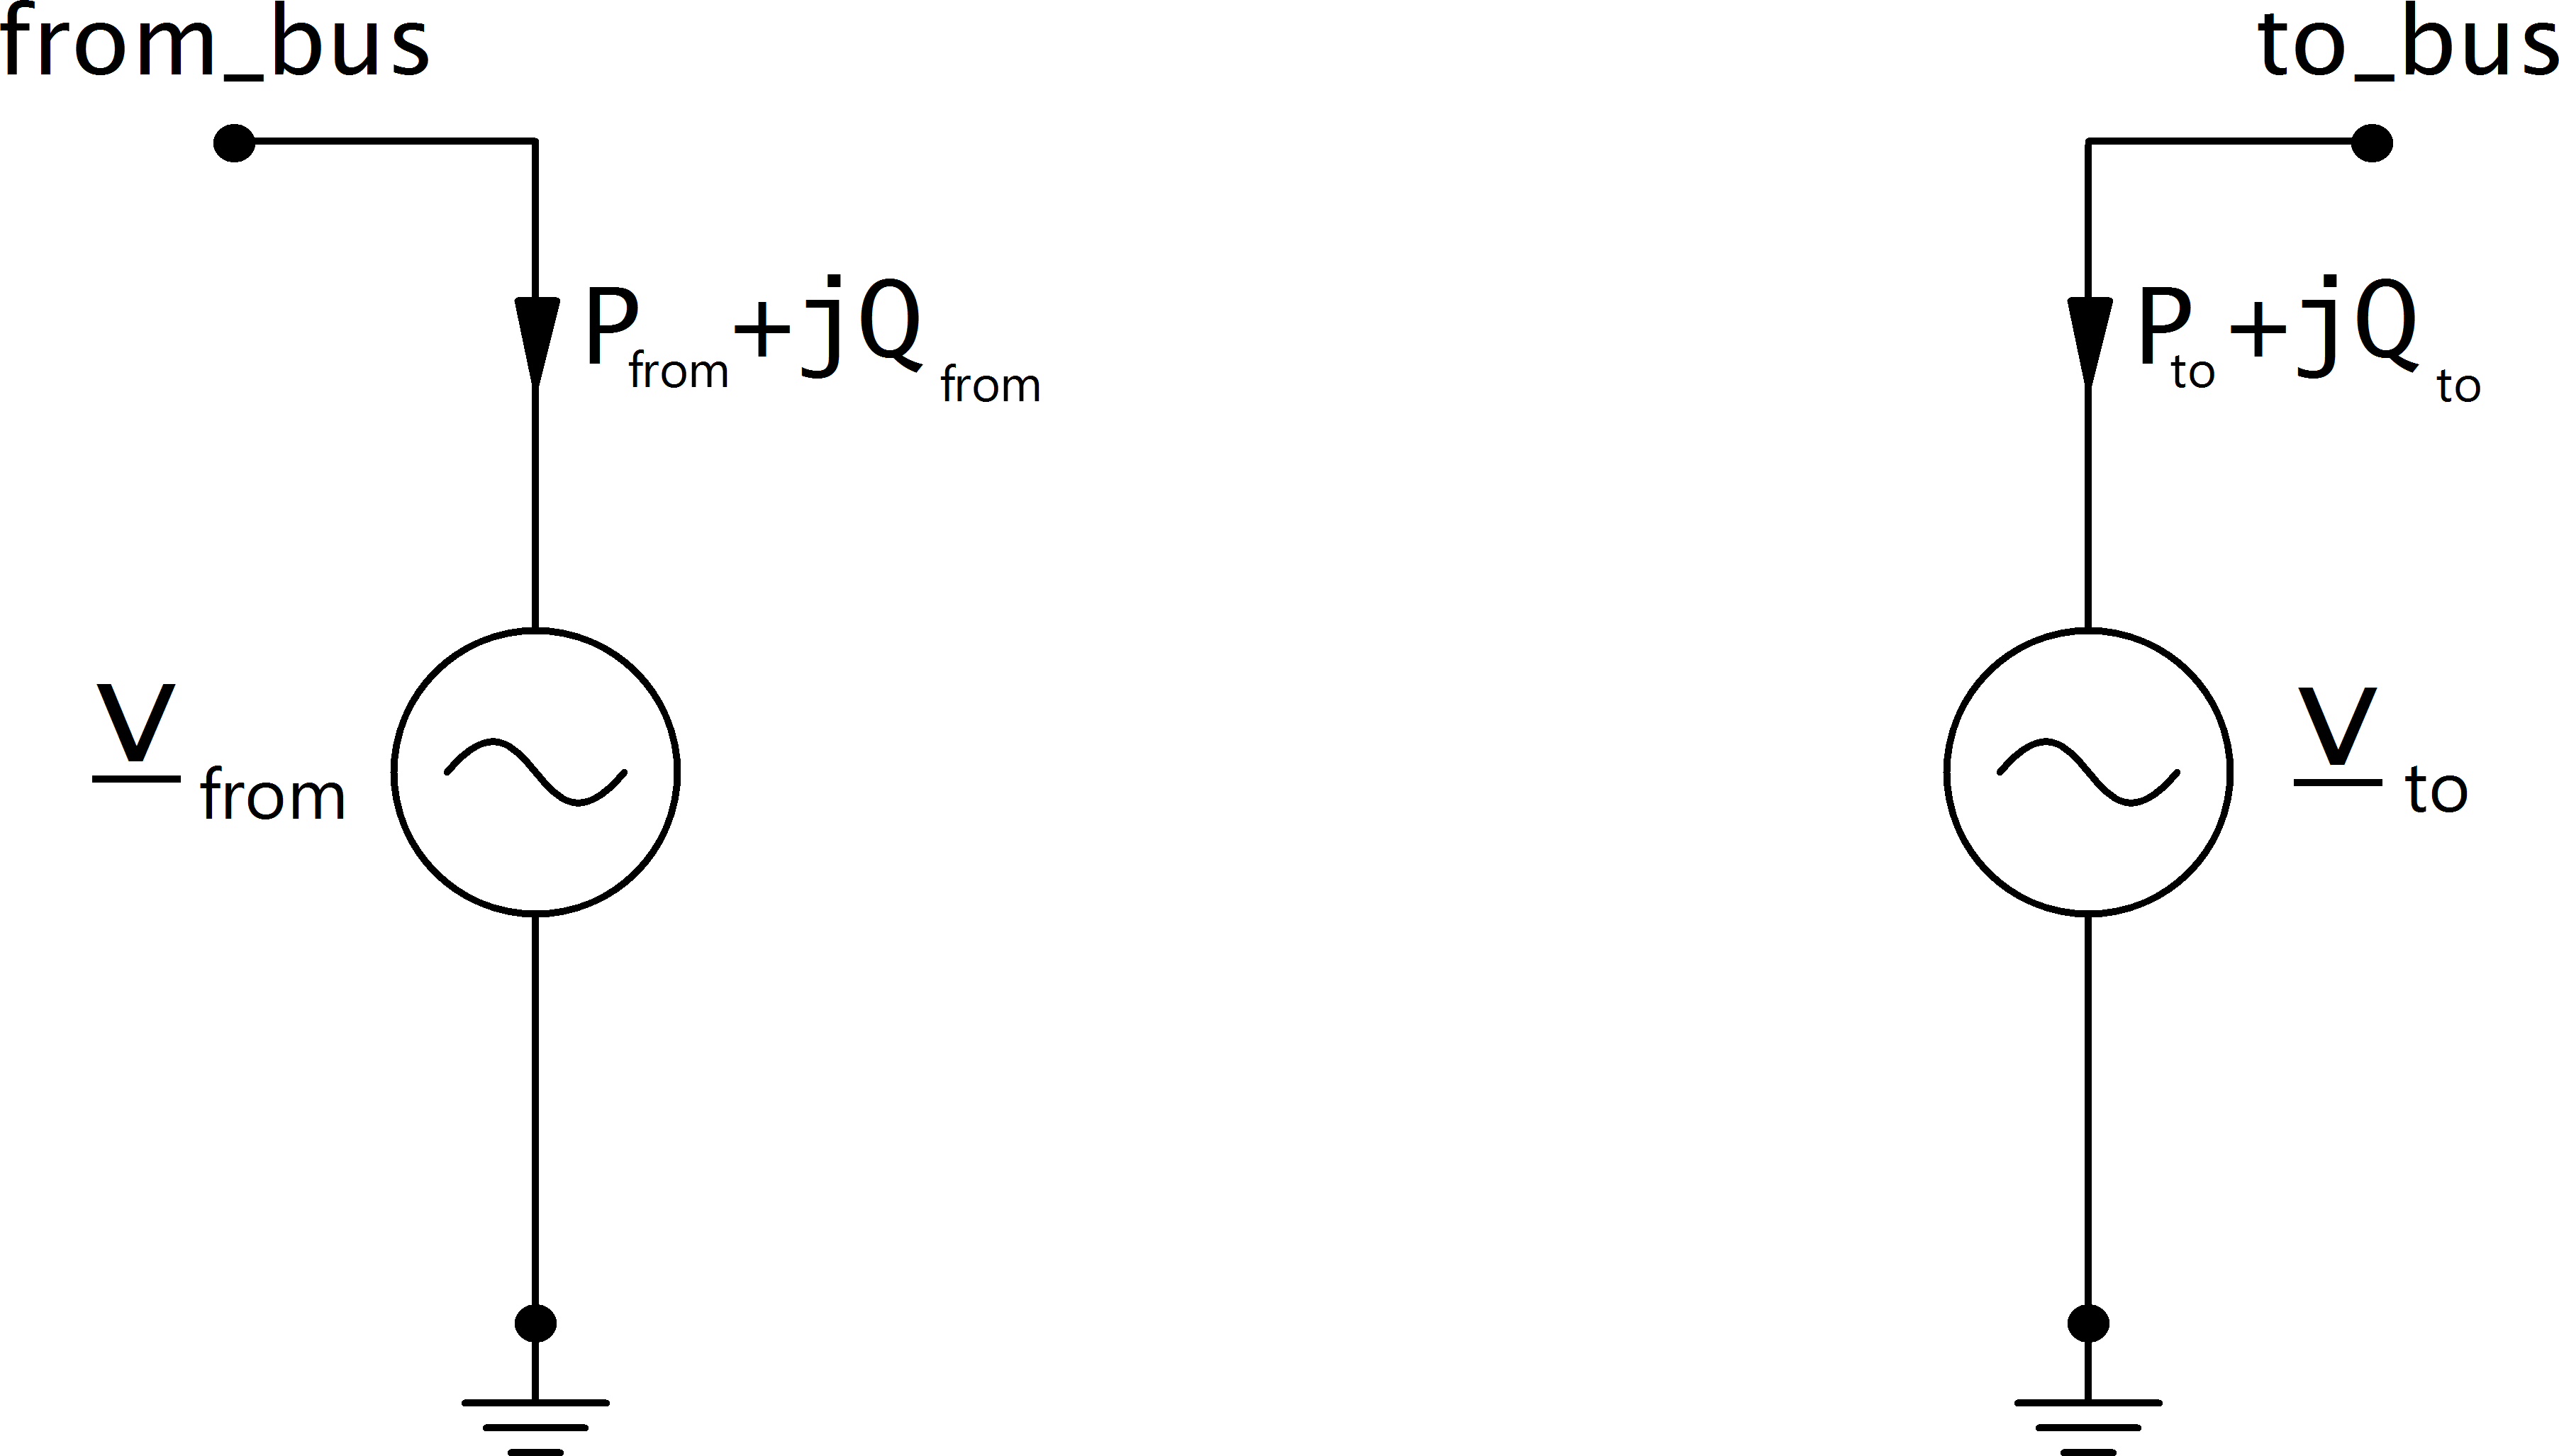
\includegraphics[width=1.0\linewidth]{images/dcline2.png}
\end{center}
\end{column}
\end{columns}

\newpage
\begin{itemize}
    \item The active power at the from side is defined by the parameters in the dcline table.
    \item The active power at the to side is equal to the active power on the from side minus the losses of the DC line.
    \item The voltage control with reactive power works just as described for the generator model. Maximum and Minimum reactive power limits are considered in the OPF, and in the PF if it is run with enforce\_q\_lims=True.
\end{itemize}

\end{frame}


\nocite{mohan2012electric, vancutsemELEC0445}


